\setcounter{secnumdepth}{-1}

\chapter{Introduction}

This report aims to complete the code that simulates a DVB-C transmission chain in matlab. It provides additional information from the theoretical part of the project and it shows the main results. \\
To simulate a transmission, each disturbance block is added and then the correction blocks are designed to compensate for the disturbances. The appropriate signals and plot are shown for each intermediate step to ensure that the blocks are working correctly. \\ 

The first step is to simulate the channel shown in figure \ref{fig:blockDiagram}. It is then followed by the addition of synchronization errors and the corresponding correction blocks. 

\vspace{2cm}

\begin{figure}[H]
    \centering
    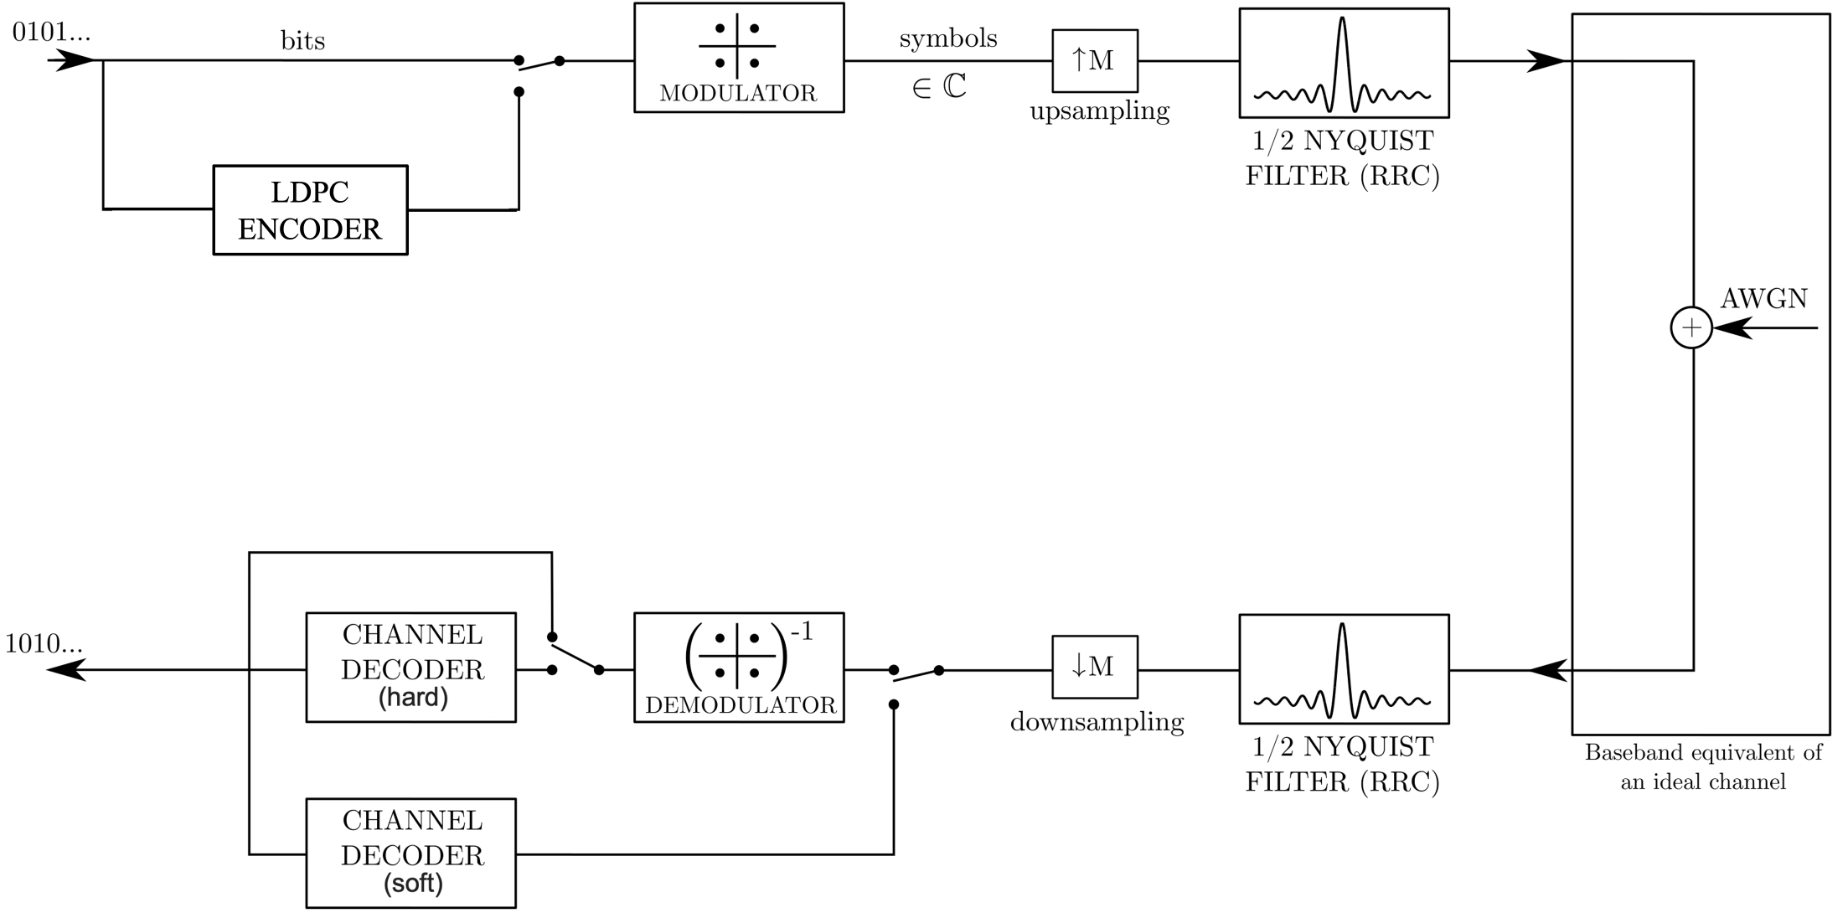
\includegraphics[width=0.9\linewidth]{blockDiagram.png}
    \caption{DVB-C transmission chain}
    \label{fig:blockDiagram}
\end{figure}
